\begin{figure}[!h]
\centering
\resizebox{\columnwidth}{!}{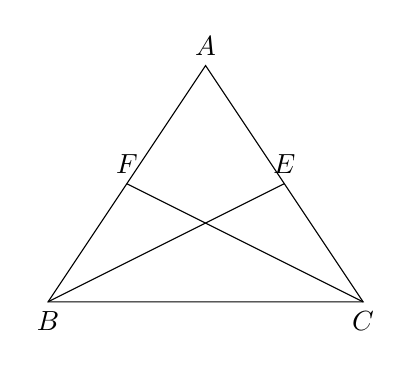
\begin{tikzpicture} 
        \coordinate (A) at (2, 3) {};
        \coordinate (B) at (0, 0) {};
        \coordinate (C) at (4, 0) {};
        \coordinate (F) at (1, 1.5) {};
        \coordinate (E) at (3, 1.5) {};
\draw (A)node[above]{$A$}--(B)node[below]{$B$}--(C)node[below]{$C$}--cycle;
\draw (B)node[below]{}--(E)node[above]{$E$};
\draw (C)node[below]{}--(F)node[above]{$F$};
\tkzMarkRightAngle[size=.2](B,E,C);
\tkzLabelAngle[dist=.5](B,E,C){};
\tkzMarkRightAngle[size=.2](C,F,B);
\tkzLabelAngle[dist=.5](C,F,B){};
\end{tikzpicture}}
\caption{Isosceles Triangle with mid-points E and F on equal sides}
\label{eq:solutions/1/16/myfig}
\end{figure}
According to figure \ref{eq:solutions/1/16/myfig}

\begin{align}
\vec{(A-B)}+\vec{(B-F)} &= \vec{(A-F)}\\
\therefore \vec{(B-F)} &= \vec{(A-F)}-\vec{(A-B)}\\
\therefore \vec{(B-F)} &= \frac{1}{2}\vec{(A-C)}-\vec{(A-B)}
\end{align}
similarly,
\begin{align}
\vec{(A-C)}+\vec{(C-E)} &= \vec{(A-E)}\\
\therefore \vec{(C-E)} &= \vec{(A-E)}-\vec{(A-C)}\\
\therefore \vec{(C-E)} &= \frac{1}{2}\vec{(A-B)}-\vec{(A-C)}
\end{align}
Since AB = AC\\
$\therefore (AB)^2 = (AC)^2$\\
\begin{align}
\therefore\norm{\vec{(A-B)}}^2 = \norm{\vec{(A-C)}}^2
\end{align}
\begin{multline}
\norm{\vec{(A-B)}}^2+\frac{1}{4}\norm{\vec{(A-C)}}^2 -\vec{(A-C)}^T\vec{(A-B)} =\\
\norm{\vec{(A-C)}}^2+\frac{1}{4}\norm{\vec{(A-B)}}^2 -\vec{(A-B)}^T\vec{(A-C)} \end{multline}
\begin{multline}
\brak{\frac{1}{2}\vec{(A-C)}-\vec{(A-B)}}^T\brak{\frac{1}{2}\vec{(A-C)}-\vec{(A-B)}}=\\
\brak{\frac{1}{2}\vec{(A-B)}-\vec{(A-C)}}^T\brak{\frac{1}{2}\vec{(A-B)}-\vec{(A-C)}}
\end{multline}
\begin{align}
\norm{\vec{(B-F)}}^2 &= \norm{\vec{(C-E)}}^2\\
\therefore\norm{\vec{B-F}} &= \norm{\vec{C-E}}
\end{align}
Hence, BF is equal to CE
